\frame{\frametitle{A Single Linear Equation}

    A linear equation has the form \pause
    \begin{equation*}
    a_1 x_1 + a_2 x_2 + \cdots + a_n x_n = b 
    \end{equation*}
    \pause
    $ a_1 ,\dotsc, a_n$ and $b$ are the \Emph{coefficients}, \pause $ x_1 ,\dotsc, x_n$ are the \Emph{variables} or \Emph{unknowns}, \pause and $n$ is the number of variables.
    
    \vspace{0.5cm} 
    
    For example, \pause
    \begin{itemize}
        \item  $2x_1+4x_2=4$ is one equation with two variables
        \item  $3x_1+2x_2+x_3=6$ is one equation with three variables
    \end{itemize}

} 


\frame{\frametitle{Systems of Linear Equations}

When we have one or more linear equation, we have a \Emph{linear system} of equations. \pause For example, a linear system with two equations is \pause
\begin{align*}
\begin{matrix}
 x_1 &+ \ 1.5 x_2 & + \ 0.9 x_3 &= \ 4
 \\[2pt]
 5 x_1 &  & + \ 7 x_3 & = \ 5
\end{matrix}
\end{align*}

\pause
We might want to know:

\pause
\begin{itemize}
    \item what values of the unknowns satisfy both equations? 
    \item what procedure can we use to identify those values? 
\end{itemize}
}

\frame{\frametitle{The Solution Set}

\vspace{4pt}
\pause 
\begin{center}\begin{tikzpicture} \node [mybox](box){\begin{minipage}{0.95\textwidth}\vspace{4pt}

    The set of all possible values of $x_1, x_2, \ldots x_n$ that satisfy all equations is the \Emph{solution set} of the system. \pause One point in the solution set is a \Emph{solution}.

    
\end{minipage}};\node[fancytitle, right=10pt] at (box.north west) {\textbf{Definition: A Solution of a Linear System}};\end{tikzpicture}\end{center}

% A system can have a unique solution, no solution, or an infinite number of solutions.

}

\frame{\frametitle{Two Variable Case}

The equation of the form $ a_1 x_1 + a_2 x_2 = b$ defines a line. How many different ways can two lines intersect? 

\begin{columns}
\begin{column}{.35\textwidth}
    \onslide<2->{\begin{align*}
    {\color{DarkRed} x_1 - 2 x_2 \, } & {\color{DarkRed} = -1} \\ {\color{Teal} -x_1 + 3 x_2 \, } & {\color{Teal} = 3 }
    \end{align*}}\vspace{-18pt}\begin{center}
    \onslide<3->{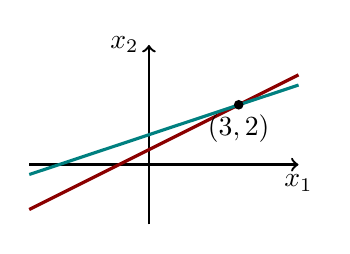
\begin{tikzpicture}[scale=0.38] 
    \draw [line width=0.30mm,->]  (-4, 0) -- (5 ,0) node[anchor=north] {$x_1$}; 
    \draw [line width=0.30mm,->]  (0,-2) -- (0, 4) node[anchor=east] {$x_2$};  
    \color{gray} 
    \draw [line width=0.40mm, DarkRed ] (-4,-1.5) -- (5,3);  \draw [line width=0.40mm, Teal ] (-4,-0.33) -- (5, 2.66);  
    \draw [black,fill=black] (3,2) circle (.4em) node[below] {$ (3,2)$};  
    \end{tikzpicture}}
    \onslide<4->{non-parallel lines \\ exactly one solution } 
\end{center}


\end{column}

    \begin{column}{.35\textwidth}
        \onslide<5->{\begin{align*}
        {\color{DarkRed} x_1 - 2 x_2 \, } & {\color{DarkRed} = -1} \\ {\color{Teal} -x_1 +2  x_2\,  } & {\color{Teal} = 1}
        \end{align*}}\vspace{-18pt}
        \begin{center}
        \onslide<6->{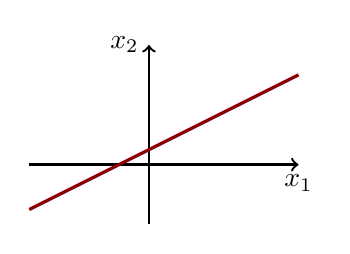
\begin{tikzpicture}[scale=0.38] 
        \draw [line width=0.30mm,->]  (-4, 0) -- (5 ,0) node[anchor=north] {$x_1$}; 
        \draw [line width=0.30mm,->]  (0,-2) -- (0, 4) node[anchor=east] {$x_2$}; 
        \color{gray} 
        \draw [line width=0.40mm, DarkRed ] (-4,-1.5) -- (5,3); 
        \end{tikzpicture}}
        \onslide<7->{identical lines \\ infinitely many solutions}
        \end{center}
    \end{column}
    
\begin{column}{.35\textwidth}
    \onslide<8->{\begin{align*}
    {\color{DarkRed} x_1 - 2 x_2\, } & {\color{DarkRed} = -1} \\ {\color{Teal} -x_1 +2  x_2\, } & {\color{Teal}= 3} 
    \end{align*}}\vspace{-18pt}\begin{center}
    \onslide<9->{
    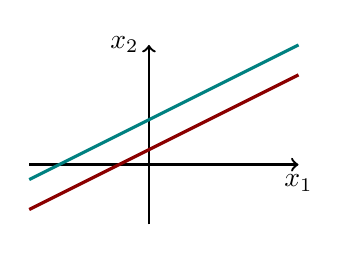
\begin{tikzpicture}[scale=0.38] 
    \draw [line width=0.30mm,->]  (-4, 0) -- (5 ,0) node[anchor=north] {$x_1$}; 
    \draw [line width=0.30mm,->]  (0,-2) -- (0, 4) node[anchor=east] {$x_2$}; 
    \color{gray} 
    \draw [line width=0.40mm, DarkRed ] (-4,-1.5) -- (5,3);  \draw [line width=0.40mm, Teal ] (-4,-0.5) -- (5, 4);  
    \end{tikzpicture}}
    \onslide<10->{parallel lines \\ no solutions}
    \end{center}
\end{column}



    \end{columns}
}


\frame{\frametitle{Three Variable Case} 

    The equation $ a_1 x_1 + a_2 x_2 + a_3 x_3 = b$ defines a plane. The \Emph{solution set} to a system of \Emph{three equations} is the set of points were all planes intersect. 
    
    \onslide<2->{How many different ways can three planes intersect? }
    
    
    % \newcolumntype{C}[1]{>{\centering\arraybackslash}m{#1}}
    \vspace{12pt}
    {\small 
    \begin{center}
        \begin{tabular}{ m{4.5cm} m{4.5cm} m{4cm}}
        \onslide<3->{
        \begin{center}planes intersect at a point\end{center} & 
        \begin{center}planes intersect on a line  \end{center}&
        \begin{center}parallel planes  \end{center}
        }
        \\[-2pt]
        \onslide<4->{
            \begin{center}
    \tdplotsetmaincoords{70}{135}
    \begin{tikzpicture}[scale=1,
        axis/.style={->,black,-stealth}, 
        solline/.style={DarkRed,thick},
        tdplot_main_coords
        ]

        \coordinate (O) at (0,0,0);
        \coordinate (X) at (1,0,0);
        \coordinate (Y) at (0,1,0);        
        \coordinate (Z) at (0,0,1);        
        \coordinate (W) at (.5,-1.8,0);        
        
        % planes
        \filldraw[draw=Teal!90,fill=Teal!15] (O) -- (Y) -- (0,1,1) -- (Z) -- cycle;
        \filldraw[draw=Teal!90,fill=Teal!15] (O) -- (X) -- (1,0,1) -- (Z) -- cycle;
        \filldraw[draw=Teal!90,fill=Teal!15] (O) -- (X) -- (1,1,0) -- (Y) -- cycle;
        
        % solution 
        \node [DarkRed] at (0,0) {\textbullet};
        
    \end{tikzpicture}
    \end{center} &
            \begin{center}
    \tdplotsetmaincoords{80}{25}
    \begin{tikzpicture}[scale=1,
        axis/.style={->,black,-stealth}, 
        solline/.style={DarkRed,very thick},
        tdplot_main_coords
        ]

        \coordinate (O) at (0,0,0);
        \coordinate (X) at (1,0,0);
        \coordinate (Y) at (0,1,0);        
        \coordinate (Z) at (0,0,1);        
        \coordinate (W) at (.5,-1.8,0);        
        
        % planes
        \filldraw[draw=Teal!90,fill=Teal!15] (O) -- (Y) -- (0,1,1) -- (Z) -- cycle;
        \filldraw[draw=Teal!90,fill=Teal!15] (O) -- (X) -- (1,0,1) -- (Z) -- cycle;
        \filldraw[draw=Teal!90,fill=Teal!15] (O) -- (1,-1,0) -- (1,-1,1) -- (Z) -- cycle;
        
        % solution line
        \draw[solline] (O) -- (Z);
        
    \end{tikzpicture}
    \end{center} & 
            \begin{center}
    \tdplotsetmaincoords{70}{135}
    \begin{tikzpicture}[scale=0.95,
        axis/.style={->,black,-stealth}, 
        solline/.style={DarkRed,thick},
        tdplot_main_coords
        ]

        \coordinate (O) at (0,0,0);
        \coordinate (X) at (1,0,0);
        \coordinate (Y) at (0,1,0);        
        \coordinate (Z) at (0,0,1);        
        \coordinate (W) at (.5,-1.8,0);        
        
        % planes
        \filldraw[draw=Teal!90,fill=Teal!15] (0,0,0) -- (1,0,0) -- (1,0,1) -- (0,0,1) -- cycle;
        \filldraw[draw=Teal!90,fill=Teal!15] (0,.5,0) -- (1,.5,0) -- (1,.5,1) -- (0,.5,1) -- cycle;
        \filldraw[draw=Teal!90,fill=Teal!15] (0,1,0) -- (1,1,0) -- (1,1,1) -- (0,1,1) -- cycle;
        
        
    \end{tikzpicture}
    \end{center} 
        }
        \\[-2pt]
        \onslide<5->{
        \begin{center} unique solution  \end{center} &
        \begin{center} infinite number of solutions  \end{center} &
        \begin{center} no solution  \end{center}\\
        }
        \end{tabular}
    \end{center}
    }
}


\frame{\frametitle{Number of Solutions} 

    \begin{center}\begin{tikzpicture} \node [mybox](box){\begin{minipage}{0.95\textwidth}\vspace{4pt}

    The solution set to a system of linear equations can only have
    \begin{itemize}
        \item<2-> exactly one point (there is a unique solution), or
        \item<3-> infinitely many points (there are many solutions), or
        \item<4-> no points (there are no solutions)
    \end{itemize}
    
    
\end{minipage}};\node[fancytitle, right=10pt] at (box.north west) {\textbf{Theorem: the Number of Solutions to a Linear System}};\end{tikzpicture}\end{center}

    \onslide<4->{Later in this course we will see why these are the only three possibilities.}
        
}


\frame{\frametitle{Row Reduction by Elementary Row Operations} 

    How can we find the solution set to a set of linear equations? 
    
    \vspace{12pt}
    We can manipulate equations in a linear system using \Emph{row operations}.
    \vspace{4pt}
    
    
    %%  ENUMERATE
    \begin{enumerate}\setlength{\itemsep}{8pt}
    \item<2->  (Replacement/Addition)  Add a multiple of one equation to another.  
    \item<3-> (Interchange)  Interchange two equations. 
    \item<4-> (Scaling) Multiply an equation by a non-zero scalar.  
    \end{enumerate}
    %% ENUMERATE
    \vspace{4pt}
    \onslide<5->{When we apply these operations to a linear system we do not change the solution set.} \onslide<6->{Let's use these operations to solve a system of equations. }
    }
    
    
    
    \frame{\frametitle{Example: Solving a Linear System} 
    
    Identify the solution set of the linear system.
    \begin{align*}
    \begin{array}{cccc}
    x_1 &  & -7 x_3 &= 8  \\
     & 2x_2 &-8x_3 &= 8 \\
     2x_1 &  & -2x_3 &= 4
    \end{array}
    \end{align*}

}




\frame{\frametitle{Summary } 
    \SummaryLine \vspace{4pt}
    \begin{itemize}\setlength{\itemsep}{8pt}
        \item systems of linear equations
        \item elementary row operations
        \item applying elementary row operations to solve a linear system
        \end{itemize}
        \vspace{4pt}
}







% \frame{\frametitle{Augmented Matrices} 

% It is redundant to write $x_1,x_2,x_3$ again and again, so we rewrite systems using matrices. For example,
% \begin{equation*}
% \begin{array}{cccc}
%     x_1 & - 2x_2 &+ x_3 &=0  \\
%  & 2x_2 &-8x_3 &= 8 
% %  5x_1 &  & -5x_3 & =10
% \end{array}
% \end{equation*}

% can be written as the \Emph{augmented matrix},

% \begin{equation*}
% \begin{amatrix}{3}
%  1 & -2 & 1 & 0 \\
%  0 & 2 & -8 & 8 
% \end{amatrix}
% \end{equation*}

% \vspace{4pt}
% The vertical line reminds us that the first three columns are the coefficients to our variables $x_1$, $x_2$, and $x_3$.
% }




% \frame{\frametitle{Consistent Systems and Row Equivalence} 

% \Emph{Definition: Consistent}\\[2pt]
% A linear system is \emph{consistent} if it has at least one solution. 

% \hspace{24pt}

% \Emph{Definition: Row Equivalence}\\[2pt]
% Two matrices are \emph{row equivalent} if a sequence of row operations transforms one matrix into the other. 

% \vspace{12pt}

% Note: if the augmented matrices of two linear systems are row equivalent, then they have the same solution set.
% %\end{block}
% } 




% \frame{\frametitle{Fundamental Questions}

% Two questions that we will revisit many times throughout our course.
% \begin{enumerate}
% \item  Does a given linear system have a solution? In other words, is it consistent? 
% \item  If it is consistent, is the solution unique? 
% \end{enumerate}
% }

    